\label{sec:tradeoff}
$S_3$ adds exactly one LLM call per ReAct episode relative to the paper's
trigger, versus the up to $n_{sc}$ additional calls incurred whenever a
back-off actually fires. The relevant comparison is therefore not the
\emph{arm's} total cost but its cost \emph{conditional on firing}: a
trigger with higher precision spends its back-off budget on episodes that
were actually wrong more often, so for a fixed back-off budget it
recovers more accuracy per dollar. Figure~\ref{fig:tradeoff} plots
accuracy against cost per question across every method and trigger arm,
with the Pareto frontier marked; a trigger degenerating toward ``always
back off'' would appear far to the right at accuracy no better than plain
CoT-SC, which the figure makes directly visible rather than requiring it
to be inferred from a table.

\begin{figure}[t]
\centering
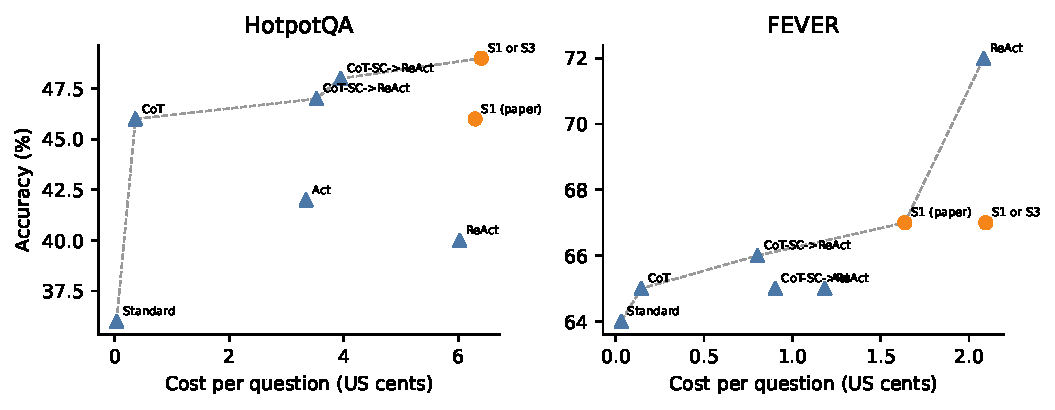
\includegraphics[width=\linewidth]{figures/fig_tradeoff.pdf}
\caption{Accuracy vs.\ cost per question (US\textcent), with Pareto
frontier (dashed).}
\label{fig:tradeoff}
\end{figure}

\begin{table}[t]
\caption{Cost per question and mean LLM calls per question, by arm.}
\label{tab:cost}
\centering\small
\begin{tabular}{@{}llrr@{}}
\toprule
Domain & Arm & Cost/q (\textcent) & Mean calls \\
\midrule
HotpotQA & ReAct$\to$CoT-SC (paper) & 6.29 & 52.5 \\
HotpotQA & ReAct$\to$CoT-SC ($S_1{\lor}S_3$) & 6.40 & 58.4 \\
HotpotQA & CoT-SC$\to$ReAct (paper) & 3.52 & 50.0 \\
HotpotQA & CoT-SC$\to$ReAct (entropy-CGA) & 3.95 & 53.2 \\
\addlinespace
FEVER & ReAct$\to$CoT-SC (paper) & 1.64 & 22.0 \\
FEVER & ReAct$\to$CoT-SC ($S_1{\lor}S_3$) & 2.09 & 37.6 \\
FEVER & CoT-SC$\to$ReAct (paper) & 0.90 & 41.1 \\
FEVER & CoT-SC$\to$ReAct (entropy-CGA) & 0.80 & 40.1 \\
\bottomrule
\end{tabular}
\end{table}
